\documentclass[11pt,preprint]{aastex}
%\documentclass{emulateapj}
\usepackage{hyperref}
%\usepackage{natbib}
%\usepackage{xspace}
\def\arcsec{$^{\prime\prime}$}
\bibliographystyle{apj}
\newcommand\degree{{^\circ}}
\usepackage{graphicx}
\usepackage{subfig}

\begin{document}

\title{Attempting to Understand Power Spectra}
\author{Lynne Jones, Peter Yoachim, {\v Z}eljko Ivezi{\'c}}



A note on some code and methods around calculating and inverting images and their related power spectral densities and auto covariance functions -- including the 1-d PSD and ACovF and structure function.

\section{Code to calculate and invert the FFT/PSD/ACovF and 1-D PSD/ACovF}

The code developed to calculate the FFT, PSD (Power Spectrum Density), and ACovF (AutoCovariance Function) of an image is available in the github repository at \url{http://github.com/rhiannonlynne/powerspectrum}. In particular, the basic functionality related to simply calculating (and inverting) these values is in the PImage class (see pImage.py). To supplement the documentation within the class, a short summary of the functionality of this class is covered here, along with some comments on the process of calculating and inverting images/FFTs/PSD/ACovFs and the corresponding 1-d PSD/ACovF.  Plotting functions specifically designed to make it easy to visualize the members of the class are available in PImagePlots, which inherits from PImage (see pImagePlots.py). The plots in this note were generated using functionality from PImagePlots.

\subsection{Forward calculation of the FFT, PSD, ACovF and 1-d PSD and ACovF}

First let's look at the forward calculation, from image through FFT, then PSD (and 1-d PSD), then onto the ACovF (and 1-d ACovF and SF). 

The fourier transform of the image (the FFT) is calculated using scipy's fftpack utilities. As we're transforming images, these are evenly sampled, finite inputs to the FFT - so the fast fourier transform code in scipy is well-suited to calculating what is essentially the DFT of the images. The FFT of the image is calculated using scipy.fftpack.fft2, and the related frequencies corresponding to each resulting pixel are calculated using scipy.fftpack.fftfreq.  

It's worth bringing up at this point that scipy's fft (and fft2) by default places the smallest frequency components (i.e. largest spatial scales) at the edges of the resulting FFT. To present a more natural image, and for purposes of calculating radial 1-d PSD and ACovF profiles, it is useful to use scipy.fftpack.fftshift to bring these small frequencies into the center of the resulting FFT. The PImage class offers the option to choose to create a series of either 'shifted' (i.e. using fftshift) or non-shifted versions of the FFT, 2-d PSD and 2-d ACovF, and will keep track of which version you're using, including using the correct (centrally-shifted) version to build the 1-d PSD and ACovF profiles. The default is to use shifted versions of the FFT, PSD and ACovF. 

The 2-d power spectrum density (2-d PSD) is then calculated by squaring the absolute value of the 2-d FFT (including both the real and imaginary components), as
\begin{equation}
2D\, PSD= \left| (R(u,v)^2 + I(u,v)^2 \right|
\end{equation}
(implemented in PImage as numpy.absolute(FFT)**2, which translates to the same calculation).  Note that even the 2-d PSD only captures the amplitude of the FFT variations; this can be generally translated to capturing variations in the intensity of the original image over the range of scales in the PSD. The locations within the image where these variations occurred is captured with the 2-d phase spectrum, which is calculated as
\begin{equation}
{\rm Phase\,spectrum} = arctan\left(I(u,v) \over R(u,v) \right)
\end{equation}
(implemented in PImage as numpy.arctan2(FFT.imag, FFT.real). This 2-d phase spectrum can be highly structured, and without the phase information preserved here, it is impossible to faithfully reconstruct the original image. 

The 2-d auto covariance function (2-d ACovF) is simply the inverse fourier transform of the 2-d PSD, calculated using scipy.fftpack.ifft2\footnote{This relationship is established by the Wiener-Khinchine (or Wiener-Khintchine) theorem, at least for a particular class of functions}.  This calculation requires some bookkeeping regarding shifted or unshifted FFT images, but this is handled by the PImage class.  Note that the auto covariance function is closely related to the auto correlation function, but is not the same - the auto correlation function is scaled by the variance, 
\begin{equation}
\rm{Auto\,Correlation\,Function} = {\rm{Auto\,Covariance\,Function} \over \sigma^2}
\end{equation}
and thus the auto correlation function is scaled between 0 and 1 (and is dimensionless), while the auto covariance function preserves the variance (and overall scale and power) in the original image (and has dimensions corresponding to the units of the original image squared). 

This brings us to the calculation of the 1-d PSD and the 1-d ACovF. Much of the calculation of these 1-d versions overlaps: the work is basically creating an azimuthally averaged, radial profile of the 2-d version of the PSD or the ACovF. The radial profiles are calculated with r=0 at the center of the image, thus the shifted version of the PSD or ACovF is used. The radial profiles are calculated relatively quickly using numpy histograms, which include weighting the radial profile by the number of pixels in each radial bin. In order to reduce noise in (and the size of) the 1-d PSD or 1-d ACovF, both the minimum number of pixels in each radial bin (min\_npix) and the minimum radial step (min\_dr) can be specified in the code. The minimum pixels consideration (min\_npix) kicks in near the center of the 2-d PSD, where the frequency scales are smallest and corresponding spatial scales are largest, and similarly at the center of the 2-d ACovF, where the spatial scales are smallest, but for min\_npix values on the order of 10 or less, this usually only affects the first few radius steps, even if min\_dr is as small as 1 pixel.  The resulting 1-d PSD or ACovF may not have uniform spacing in the radial profile, but the information on the step size is preserved in either frequency or spatial values corresponding to each 1-d radial profile data point. 

Finally, the structure function (SF) is generated from the 1-d ACovF by 
\begin{equation}
SF = SF_\infty \left( 1 - {ACovF \over \sigma^2} \right),
\end{equation}
but here the complication is that we don't really know $SF_\infty$ because our original image was of a limited size. In practice, then we calculate 
\begin{equation}
SF(r<R) = SF_R  \left( 1 - {ACovF(r<R) \over \sigma^2} \right),
\label{eq:SFsq}
\end{equation}
where $R$ is the maximum radius of the ACovF in the original image. In addition, the $SF_R$ is assumed to be equal to $\sigma^2$, and $SF(0) = 0$, so this can be simplified to 
\begin{equation}
SF = \left( ACovF(0) - ACovF \right).
\end{equation}
Note that the units of the structure function are the square of the units of the original image -- this is the typical form of the SF which is presented in statistics. However, astronomers usually show and use a modified definition of the structure function, which is simply the square root of the version above (this keeps the units of the SF the same as the units in the original image). The PImage class  uses this convention, calculating and displaying 'structure function' as the $\sqrt{SF}$ as defined in equation~\ref{eq:SFsq}, meaning that the SF as presented will be
\begin{equation}
SF = \sqrt{ACovF(0) - ACovF }. 
\label{eq:SF}
\end{equation}
Note also that a 1-d linear interpolation is used to create this SF with evenly binned spacing from the center of the image to the edge. 

Two other methods are available that can be useful for this calculation: the image can be zero padded at its edges and a hanning filter can be applied. The hanning filter gradually scales the image from its normal peak values down to 0 at $r=r_{max}$, where $r_{max}$ is user definable (the default is the edge of the image). Without the hanning filter, any discontinuities at the edges of the original image (even if the image is zero padded - there is still a discontinuity between the image values and the zero values in the padding region) will result in noise in the FFT and PSD. This is most noticeable in the PSD, as this is typically viewed on a log scale, and in the phase spectrum. Vertical and horizontal lines in the 2-d PSD aligned with the u/v axis are a typical indicator of this noise.  An example of this entire forward process is shown in Figures~\ref{fig:example_lines_a} and \ref{fig:example_lines_b}, both with and without the hanning filter\footnote{Larger sizes of these images are available in the github repository, along with code (powers\_qs.py) which will recreate all figures in this note from scratch.}.  
%While the falloff due to the hanning filter is visible in the 1-d ACovF, I believe this could be compensated for, as the window function of the hanning filter is known. 

\begin{figure}[htbp]
\centering
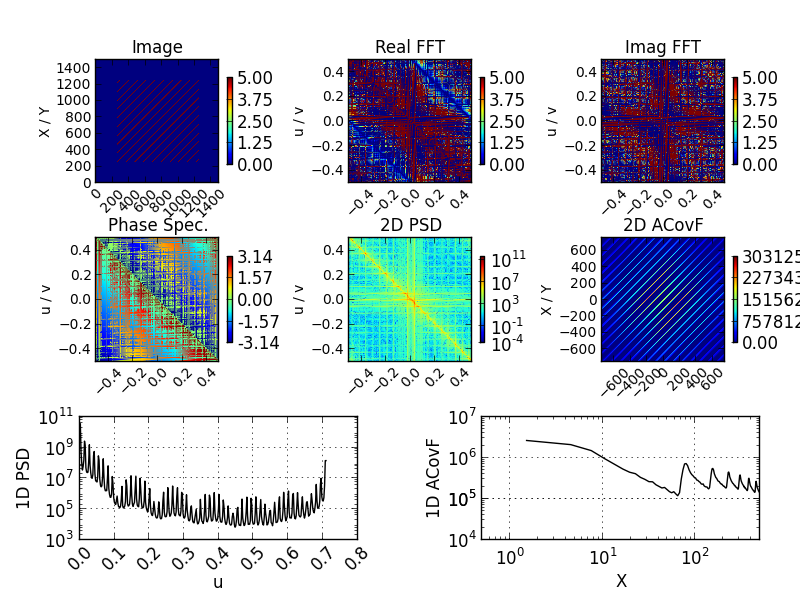
\includegraphics[width=4.2in]{example_lines_a}
\caption{{\small
Example of FFT, PSD, and ACovF calculation from a simple image, including the 1-d PSD and 1-d ACovF.  This example starts with a simple image filled with lines at a 45 degree angle, with zero padding around the outside of the image.  }}
%Figure~\ref{fig:example_lines_b} shows a similar example, but adding a hanning filter before zero padding the image. }}
\label{fig:example_lines_a}
\end{figure}

\begin{figure}[htbp]
\centering
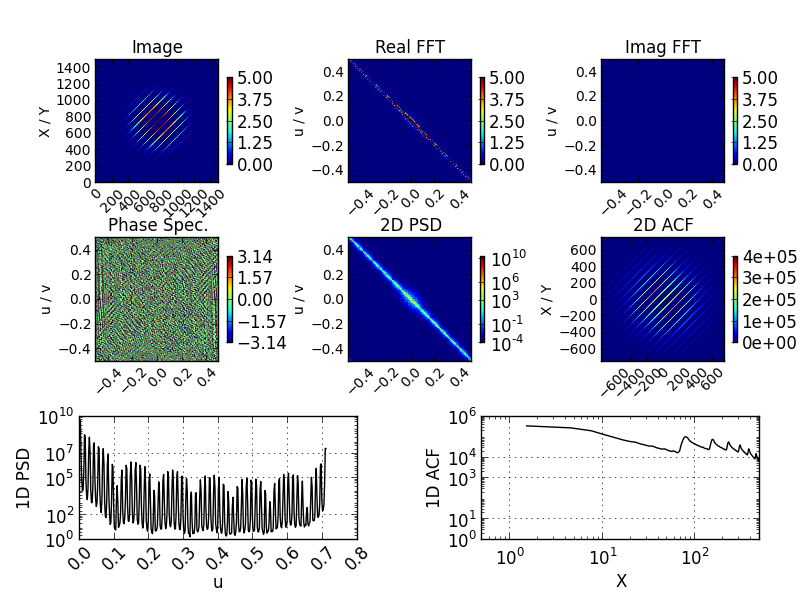
\includegraphics[width=4.2in]{example_lines_b}
\caption{{\small
Adding a hanning filter. This example is similar to Figure~\ref{fig:example_lines_a}, except a hanning filter has been applied before zero padding the image. The FFT and 2-d PSD are much cleaner (and closer to the true result which would be achieved if the image was infinitely large) with the hanning filter applied. }}
 \label{fig:example_lines_b}
\end{figure}


\subsection{Gaussian example}

Walking through the transformations of a 2-d gaussian is illustrative, because the 2-d gaussian has an analytical solution to the FFT and on down the chain to the 2-d ACovF.  An overview of the 2-d FFT, 2-d PSD and 2-d ACovF, along with the 1-d PSD and ACovF is shown in Figure~\ref{fig:gauss_all}. 

\begin{figure}[htbp]
\centering
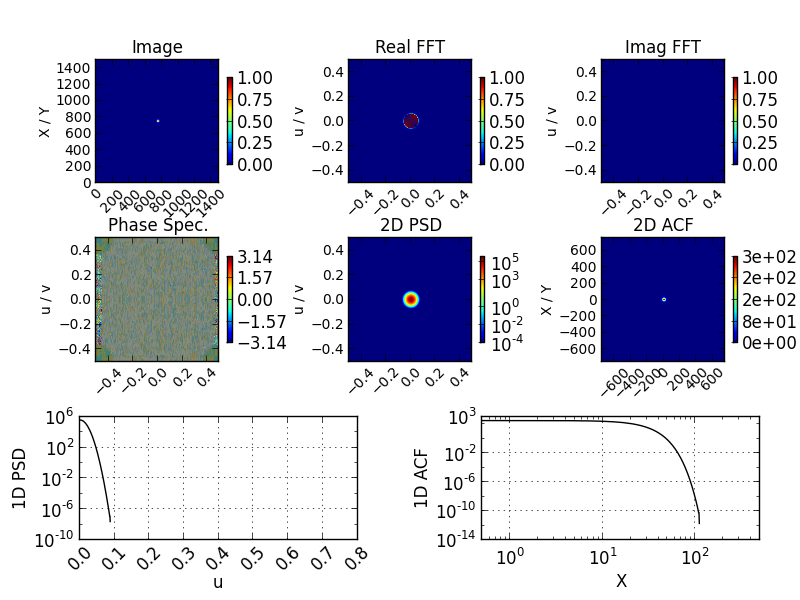
\includegraphics[width=5in]{gauss_all}
\caption{{\small
Calculation of the FFT, PSD and ACovF for a 2-d Gaussian in the input image. }}
\label{fig:gauss_all}
\end{figure}

To explore this further, however, we can look at slices through the center of the 2-d images, to compare the expected analytical representations of the gaussian as it translates from original image to FFT to 2-d PSD and to 2-d ACovF with the actual calculated widths of the gaussian. This makes sure that the scale of our various `images' (of the FFT/PSD/ACovF) are understood, particularly as we translate in and out of frequency space. In theory, the peak of the gaussian in each case should be calculable as well. In practice, I did not try to predict the peaks and instead just used the maximum value of the calculated values as the `expected' peak. (Predicting this may be a to-do, but understanding the overall structure and spatial scaling is a higher priority). 

Following along with the panels in Figure~\ref{fig:gauss_slices}: 
\begin{itemize}
\item{Panel a shows a slice through the center of the original image, where we see a gaussian with a width of $\sigma_{x}$. }
\item{Panel b shows a slice through the center of the real part of the FFT, where we see a gaussian with a width of $\sigma_{fft} = 1 / (2 \pi \sigma_{x}))$. This is as expected - the FFT of a gaussian is another gaussian, with this predicted width. Note that the $x$ axis units here are in frequency.}
\item{Panel c shows a slice through the center of the 2-d PSD, which is created by squaring the FFT. Since the square of a gaussian is another gaussian with width reduced by $\sqrt 2$, we expect $\sigma_{psd} = \sigma_{fft} / \sqrt 2$. Note that this is still in frequency space. }
\item{Panel d shows a slice through the center of the 2-d ACovF, which is created by taking the inverse FFT of the PSD. Thus we expect $\sigma_{act} = 1 / (2 \pi \sigma_{psd}) = \sigma_{x} * \sqrt 2$. Note that now we are back in pixel space, where each pixel corresponds to the same spatial scale as the original image.}
\end{itemize}
In each case, the expected width of the gaussian matches the fitted $\sigma$ values, as can be seen in the plots. 

\begin{figure}[htbp]
\centering
\subfloat[]{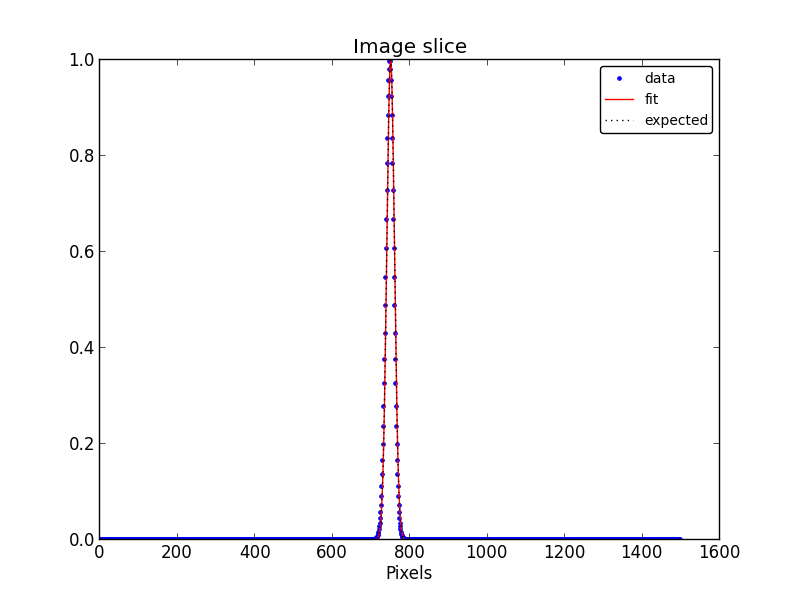
\includegraphics[width=3in]{gauss_image}}
\subfloat[]{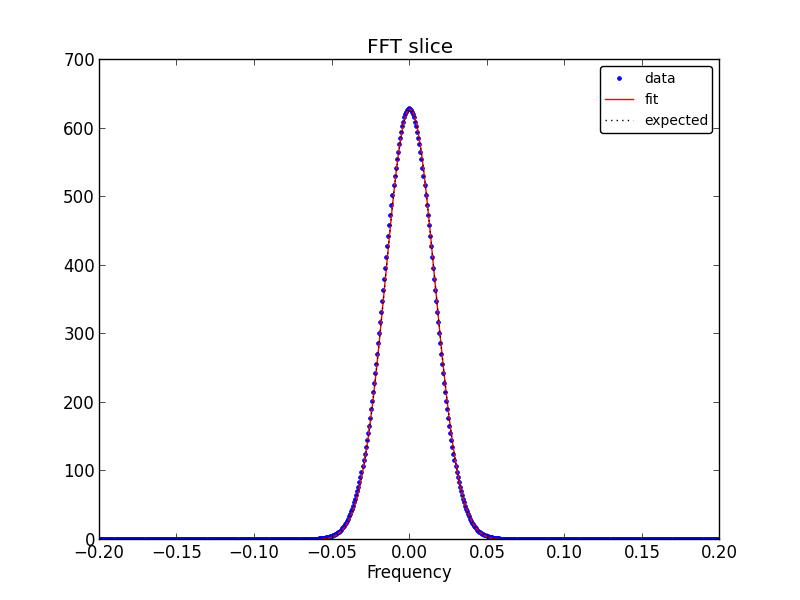
\includegraphics[width=3in]{gauss_fft}} \\
\subfloat[]{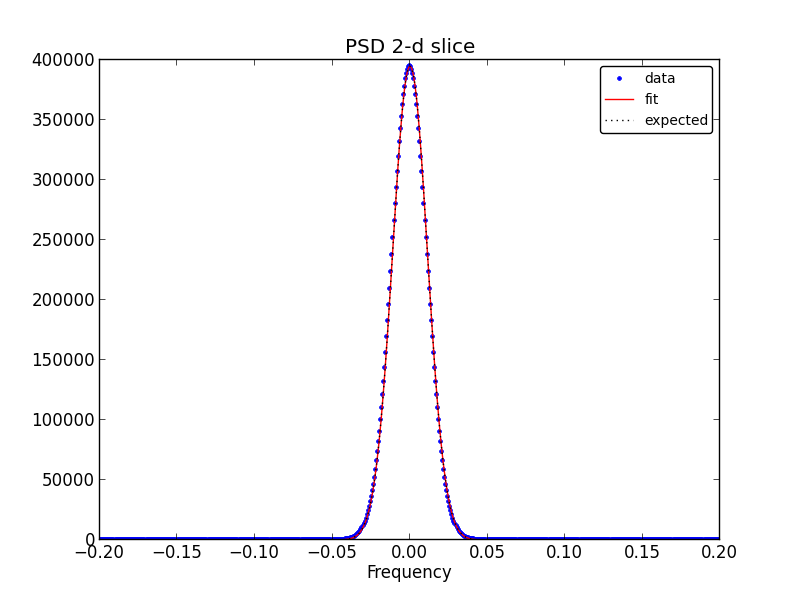
\includegraphics[width=3in]{gauss_psd_freq}}
\subfloat[]{\includegraphics[width=3in]{gauss_ACovF}}
\caption{{\small
Analyzing the forward transformations of a gaussian image. By taking slices through the center of the 2-d images representing the original image (panel a), the FFT (panel b), the PSD (panel c), and the ACovF (panel d), the expected width of the gaussian as translated to the FFT/PSD/ACovF can be compared with the actual calculated result. In each panel, the data (the calculated values) are represented by the blue dots, the analytical or expected result is plotted with the dotted black line, and a gaussian fit to the data points is shown with the red line. In all these cases, the fitted gaussian agrees very well with the expected values.}}
\label{fig:gauss_slices}
\end{figure}

We can also compare the 1-d PSD and 1-d ACovF to these expected values, to ensure that the creation of the radial profile was accurate. Figure~\ref{fig:gauss_1d} shows the results of these comparisons, where once again the expected $\sigma$ values are recovered from the 1-d profiles. 

\begin{figure}[htb]
\centering
\subfloat[]{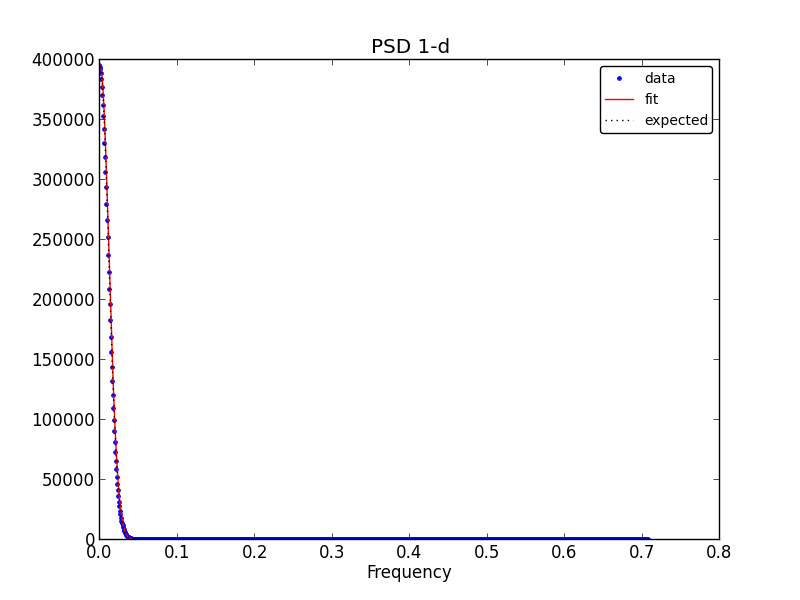
\includegraphics[width=3in]{gauss_psd1d}}
\subfloat[]{\includegraphics[width=3in]{gauss_ACovF1d}}
\caption{{\small
The 1-d PSD and ACovF profiles for a gaussian image. These plots show a comparison of the calculated values of the 1-d PSD (panel a) and 1-d ACovF (panel b) with the result expected from the gaussian distribution and the azimuthal symmetry of the 2-d cases of the PSD and ACovF. The blue circles represent the calculated values, while the expected result is plotted as a dotted black line, while a gaussian fit to the data points is shown with the red line.  This shows that the 1-d calculation preserves the expected radial profile. }}
\label{fig:gauss_1d}
\end{figure}


There is one case which is somewhat perplexing, although I think this is actually just related understanding what the 1-d PSD actually means. The 1-d PSD in frequency space matches expectations for this gaussian, but it is also possible to translate this profile from frequency space back to the original (or physical) pixel space. Panel a in Figure~\ref{fig:gauss_psd_spatial} illustrates how this is possible, by taking a slice through the center of the 2-d PSD and translating the width of the gaussian in pixel coordinates in the 2-d PSD image to the width of the gaussian in frequency coordinates -- $\sigma_{psd(pix)} = \sqrt{n_x\, n_y} / (2 \pi \sigma_{psd(freq)}$ (note that this is generally what we would expect from an FFT, with the addition of the $\sqrt{n_x\,n_y}$ term). If we then calculate the 1-d PSD and translate the frequency values into pixel coordinates using a similar formula -- $x = \sqrt{n_x\,n_y} / (2 \pi freq)$ -- then we obtain the 1-d PSD in pixel / physical values, as is shown in panel b of Figure~\ref{fig:gauss_psd_spatial}.  The perplexing part of this is knowing what to expect for this 1-d PSD in pixel values; the result is no longer gaussian. Even trying to match a gaussian distribution with $\sigma_{psd(pix)}$ to this profile and compensating for the shift from frequency to pixels doesn't match the data points. This raises the question of whether trying to interpret the 1-d PSD in pixel (or original/physical scale) coordinates is meaningful, whether any interpretation attached to the original spatial scales should be done using the 1-d ACovF instead (which naturally exists in pixel scales and does match what intuition would suggest), or whether the problem is simply that `intuition' isn't leading us to the right conclusions here and simply having more experience with 1-d PSD's in physical units would make this understandable. An example of the 1-d PSD in physical coordinates vs. the 1-d ACovF in physical coordinates for two comparison input images with a much different but still high degree of structure is given in Figure~\ref{fig:1d_psd_ACovF}; looking at these two comparisons illustrates the differences between what is represented in the 1-d PSD vs the 1-d ACovF.  \label{q:1dpsd}

\begin{figure}[htpb]
\centering
\subfloat[]{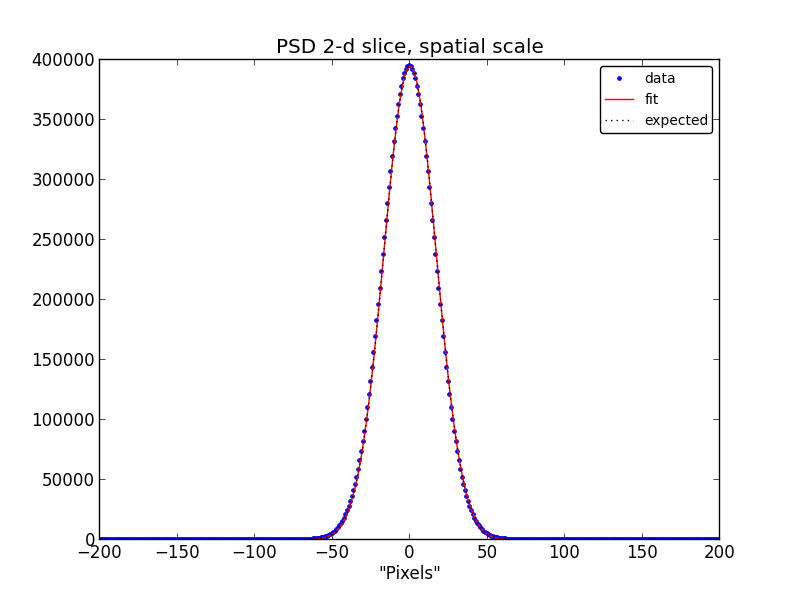
\includegraphics[width=3in]{gauss_psd_x}}
\subfloat[]{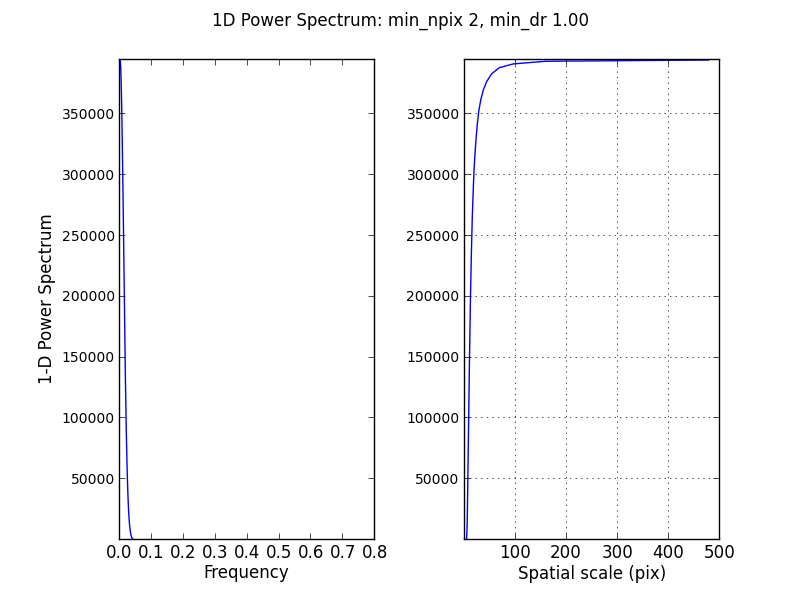
\includegraphics[width=3in]{gauss_psd1d_all}}
\caption{{\small
An analysis of the physical scaling of the 1-d PSD. Panel a shows a slice through the 2-d PSD, where the $x$ axis has been left in pixels (pixels in the 2-d PSD image), centered on 0. The gaussian fitted (red line) through the data points (blue circles) has a width $\sigma_{psd(pix)} = \sqrt{n_x\, n_y} / (2 \pi \sigma_{psd(freq)}$). Panel b shows the calculated 1-d PSD, in both frequency ($u$) and equivalently-scaled pixel coordinates ({\it i.e.} $x = \sqrt{n_x\,n_y} / (2 \pi freq)$ units.}}
\label{fig:gauss_psd_spatial}
\end{figure}

\begin{figure}[htpb]
\centering
\subfloat[]{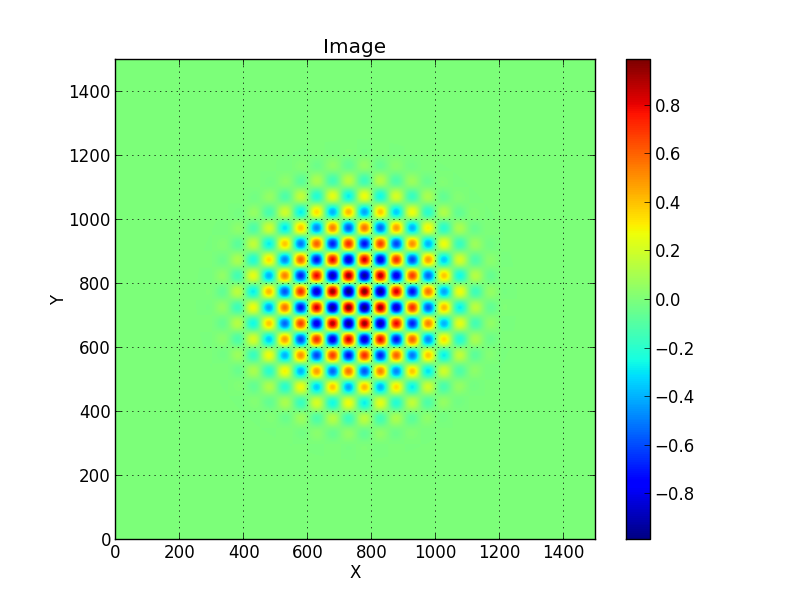
\includegraphics[width=2.4in]{compare1d_image1}}
\subfloat[]{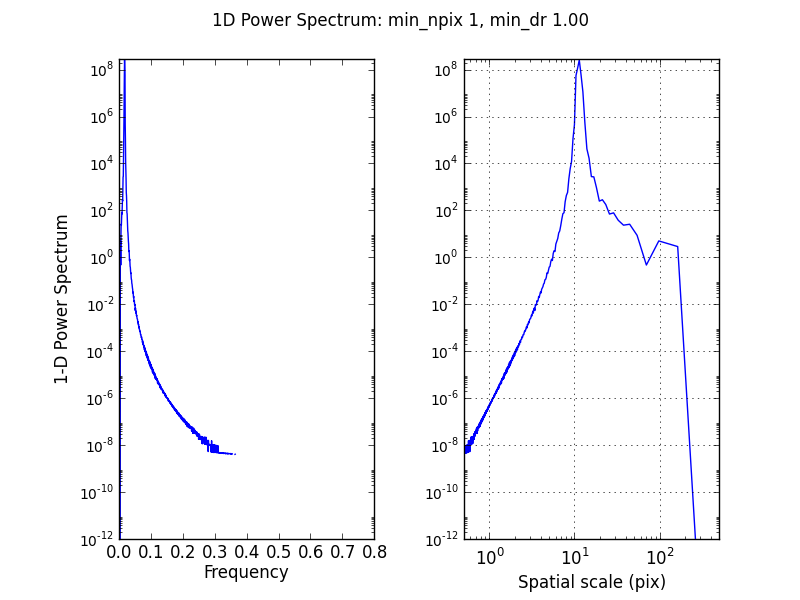
\includegraphics[width=2.5in]{compare1d_psd1}}
\subfloat[]{\includegraphics[width=2.4in]{compare1d_ACovF1}} \\
\subfloat[]{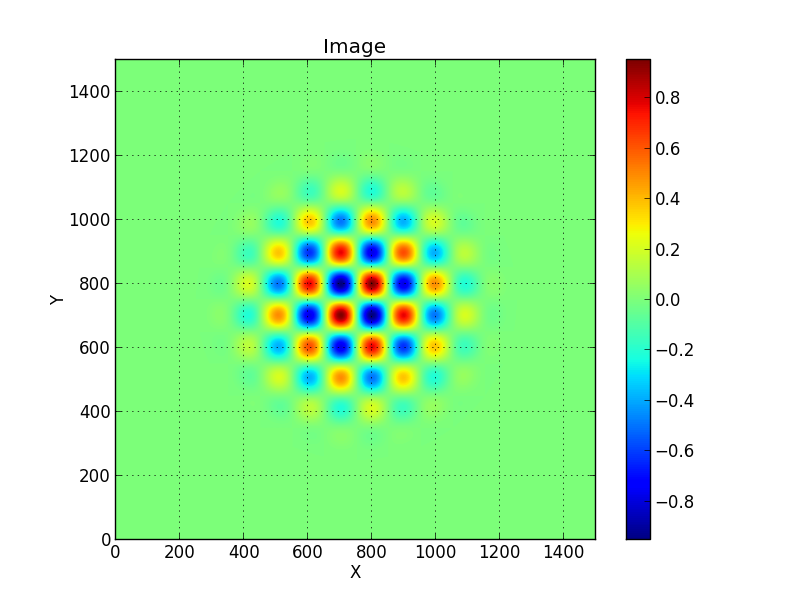
\includegraphics[width=2.4in]{compare1d_image2}}
\subfloat[]{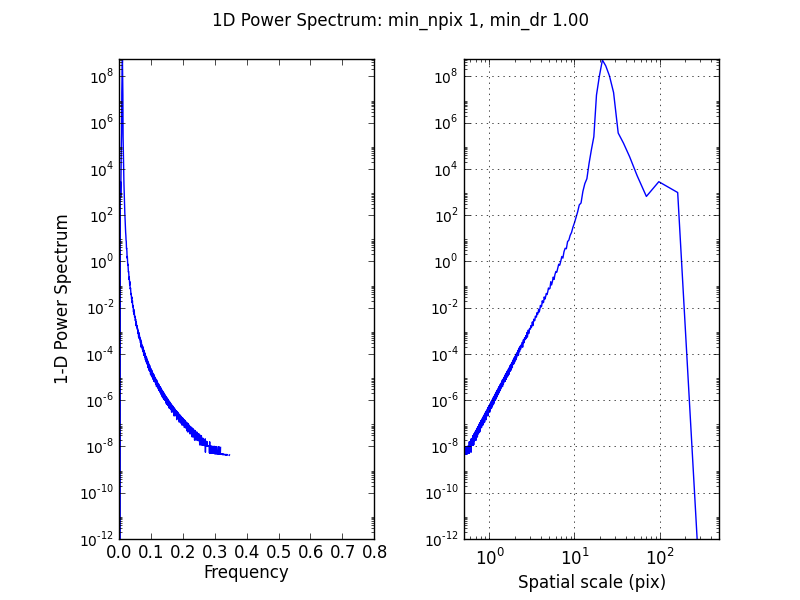
\includegraphics[width=2.5in]{compare1d_psd2}}
\subfloat[]{\includegraphics[width=2.4in]{compare1d_ACovF2}}
\caption{{\small 
A comparison of the 1-d PSD and 1-d ACovF. The top row (panels a, b, c) show the transformation of the image (panel a) into the 1-d PDS (in both frequency and physical pixel space) (panel b), and onto the 1-d ACovF (panel c). The bottom row (panels c, e, f) are similar, but start with the image in panel d, where the scale of the varying sinusoidal pattern has been doubled (the `spots' are twice as big). The result of this scaling can be seen in both the 1-d PSD and 1-d ACovF. In the 1-d PSD, the difference shows up only as a shift in the peak, by a factor of two, but the location of the peak is consistent with about half the size of the `spots' in the original image, and does match the start of the rolloff in the smallest-scale correlations in the 1-d ACovF. With the 1-d ACovF, the peaks and valleys in the image show up as regions of correlated values, so we see peaks in the ACovF at all of the regions we would naively expect from the image ({\it i.e.} within one spot and from each spot to each of the other spots at varying distances), and we see this pattern become twice as large in the lower row as in the top row. }}
\label{fig:1d_psd_ACovF}
\end{figure}


\section{Inverting the FFT, PSD, ACovF or SF to reconstruct an image}

After explaining the forward calculation of the FFT (real and imaginary), 2-d PSD and 2-d ACovF, now let's look at the various possible steps of inverting this process to reconstruct an image. This process is also handled by the PImage class. The general idea is that the inverted (or reconstructed) version of the image (or FFT or PSD or ACovF) is stored in the class with a suffix `I' -- thus the original image is `image' while the image which is reconstructed as a result of inverting the FFT is called `imageI'.  The most complicated part of this inversion process is keeping track of what you started with -- obviously, starting with a 1-d ACovF or 1-d PSD (vs. the 2-d PSD or ACovF) and with or without the phase spectrum information makes a big difference to the final reconstructed image! 

Inverting from the FFT (using both the real and imaginary components) to an image is simple using scipy.fftpack.ifft2, and recreates an almost perfect (within numerical error) image. Similarly, starting from the 2-d PSD or the 2-d ACovF plus the phase spectrum results in an almost perfect reconstruction of the original image, including the intensity scales of the original image. No information is lost as long as the phase spectrum {\it and} the 2-d PSD or ACovF is maintained. Note that if you start from the ACovF, you must first reconstruct the PSD and then the FFT and then finally the image itself, while if you start from the PSD, you just reconstruct the FFT and then the image. Examples of these `perfect' reconstructions are given in Figure~\ref{fig:invert_perfect}. 

\begin{figure}[htpb]
\centering
\subfloat[]{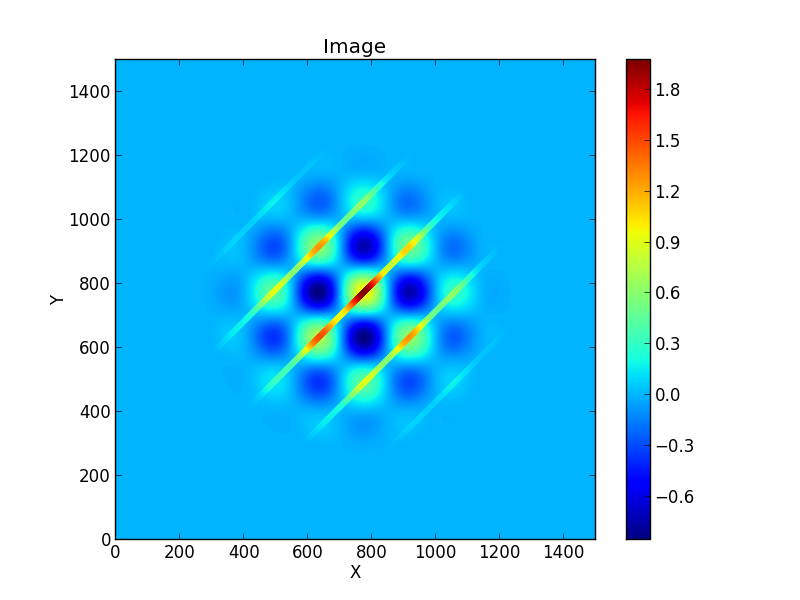
\includegraphics[width=2.4in]{invert_image}}
\subfloat[]{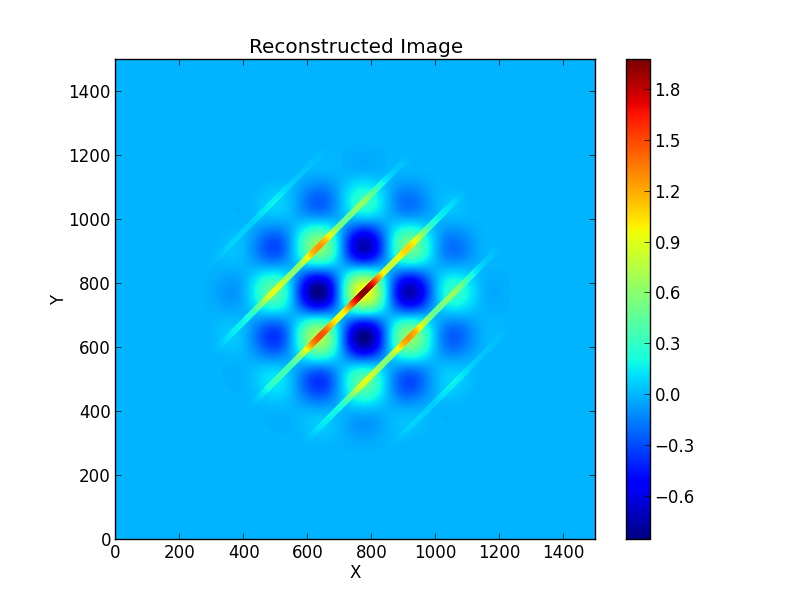
\includegraphics[width=2.4in]{invert_psd2d_good}}
\subfloat[]{\includegraphics[width=2.4in]{invert_ACovF2d_good}}
\caption{{\small
Reconstructing an image without losses. Reconstructing an image (panel a) from the 2-d PSD plus phase spectrum (panel b) and reconstructing the same image from the 2-d ACovF plus phase spectrum (panel c). By retaining the 2-d PSD or ACovF, plus the phase spectrum, the original image can be reconstructed to very high accuracy.  A hanning filter has been applied to the original image here, although in practice these images could be reconstructed perfectly well without this filter. However, applying the hanning filter here allows for a better illustration of the recovery of the 1-d PSD and 1-d ACovF in Figure~\ref{fig:invert_compare1d} below, while still keeping the input images identical.}}
\label{fig:invert_perfect}
\end{figure}

At this point, we can consider how much information is lost by attempting to reconstruct the original image (a) without the phase information but with the 2-d PSD or ACovF (keeping any azimuthal information from the PSD or ACovF, but losing the location information from the phase spectrum), (b) with the phase information but using only a 1-d PSD or ACovF (keeping the location information from the phase spectrum, but losing any azimuthal dependence from the PSD or ACovF and replacing this with a radially symmetric function), or (c) without the phase information and using only a 1-d PSD or ACovF.  Examples of these reconstructions are given in Figure~\ref{fig:invert_psd} and \ref{fig:invert_ACovF}. 

Within the PImage class, the 1-d PSD or 1-d ACovF is translated into a 2-d version by simply creating an azimuthally symmetric 2-d version of the 1-d values. The maximum $x/y$ limits of the 2-d representation will match the maximum $R$ value of the 1-d  function. The corners of the 2-d representation, beyond the range of the 1-d representation, will be filled with the value of the 1-d curve at $r=R$.  When inverting from the SF (as defined in equation~\ref{eq:SF}), the 1-d ACovF is first calculated as 
\begin{equation}
ACovF = (SF_R)^2 - SF^2.
\end{equation}
To some extent, the amount of information `lost' will depend on the input image; images which produce a nearly radially symmetrical 2-d PSD or ACovF, for example, will not suffer as strongly when the 1-d PSD or ACovF is used instead of the 2-d version. Losing the phase spectrum and replacing it with a uniformly distributed random sample of phases will generally spread the sources around the image and also modifies the intensity in the original image (although the mean value remains the same). 

In general starting from the 2-d PSD or ACovF with a random phase spectrum yields similar results. However, a comparison of inversions starting from the 1-d PSD or 1-d ACovF show differences. Starting from the 1-d ACovF preserves structure at large scales better than starting from the 1-d PSD, while starting from the 1-d PSD preserves structure at small scales better than starting from the 1-d ACovF. These are small differences, but are visible in the 1-d ACovF or PSD calculated from the reconstructed images.  This difference is partly the result of how the 1-d PSD and 1-d ACovF are calculated; because these are radial profiles, and there are only so many pixels near the very center of the image, the resolution of the 1-d ACovF is lowest at the center of the 2-d ACovF (equivalent to small spatial scales). Conversely, the resolution of the 1-d PSD is lowest at the center of the 2-d PSD, which is equivalent to the largest spatial scales. 

\begin{figure}[htpb]
\centering
\subfloat[]{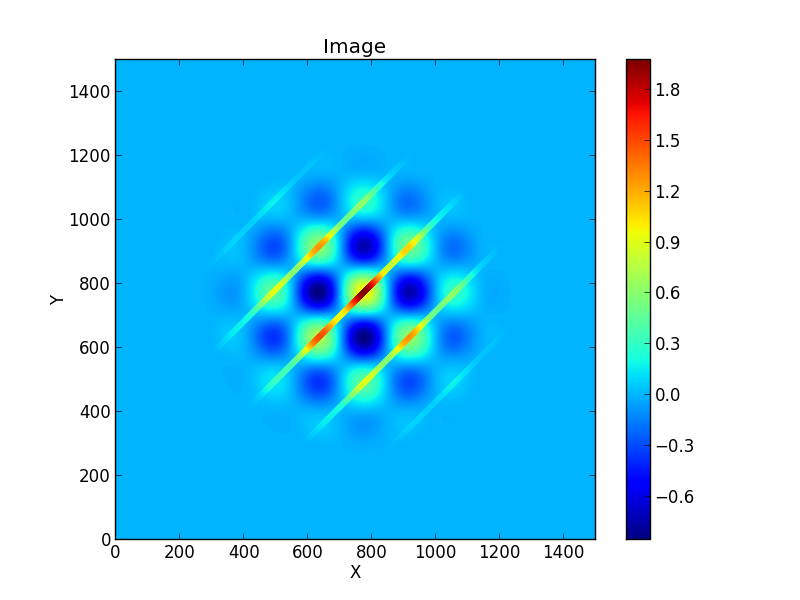
\includegraphics[width=3in]{invert_image}}
\subfloat[]{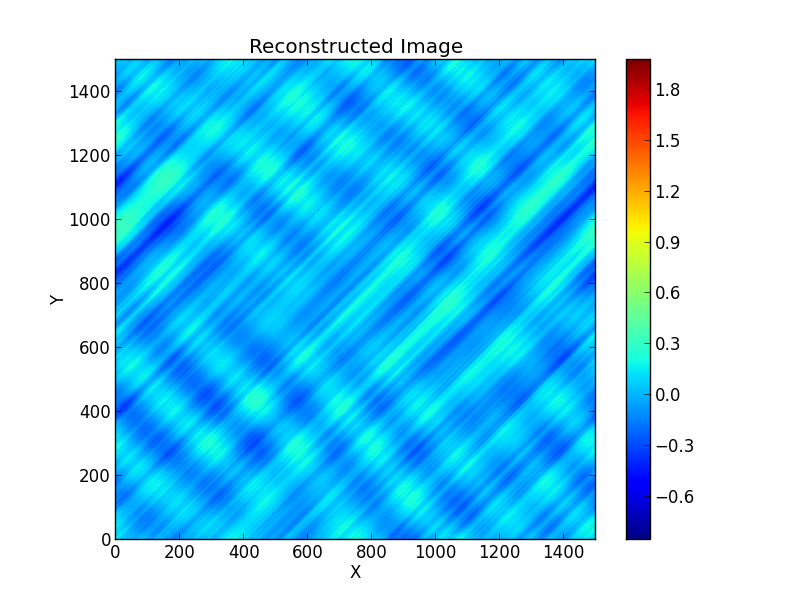
\includegraphics[width=3in]{invert_psd2d_nophases}} \\
\subfloat[]{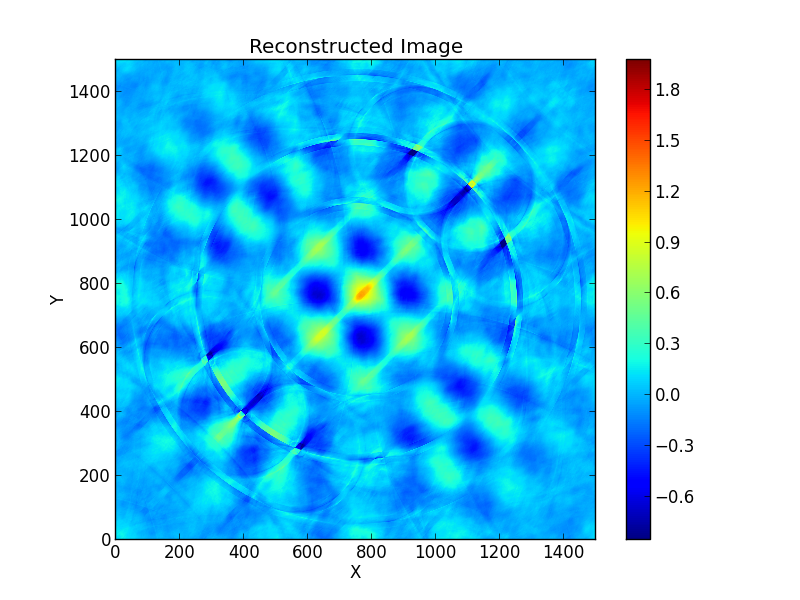
\includegraphics[width=3in]{invert_psd1d_phases}}
\subfloat[]{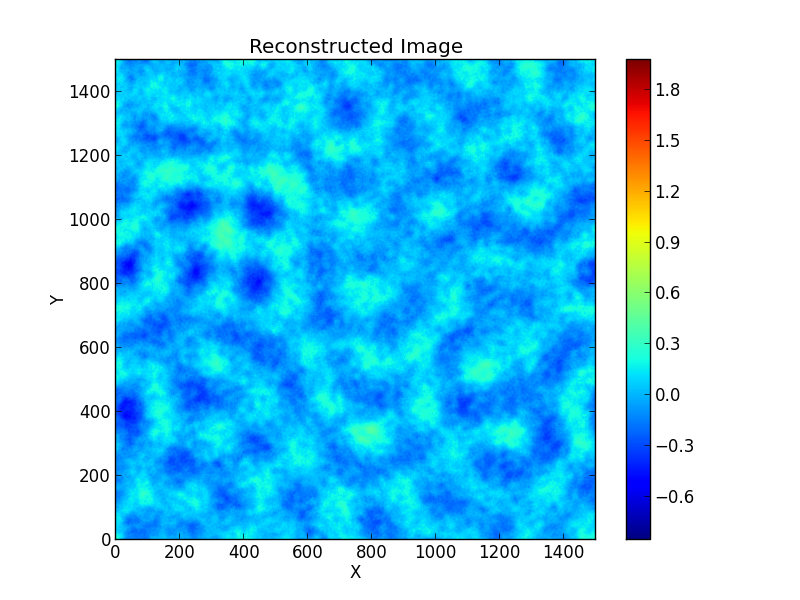
\includegraphics[width=3in]{invert_psd1d_nophases}}
\caption{{\small
Reconstructing an image after losing information, using the PSD. 
Panel a shows the original image. Panel b shows the image as reconstructed using the 2-d PSD but a uniform random distribution of phases in the phase spectrum. Panel c shows the image as reconstructed using the 1-d PSD but keeping the phase spectrum. The influence of the hanning filter is visible in the circular pattern seen in this reconstructed image -- it seems that since the function of the hanning filter is known, this should be possible to remove during the reconstruction (perhaps when doing the inverse FFT to the image), but I did not investigate this possibility. Panel d shows the image as reconstructed using the 1-d PSD and a uniform random distribution of phases (the most information loss). In all cases, the generation of the random distribution of phases was started with the same random seed. }}
\label{fig:invert_psd}
\end{figure}

\begin{figure}[htpb]
\centering
\subfloat[]{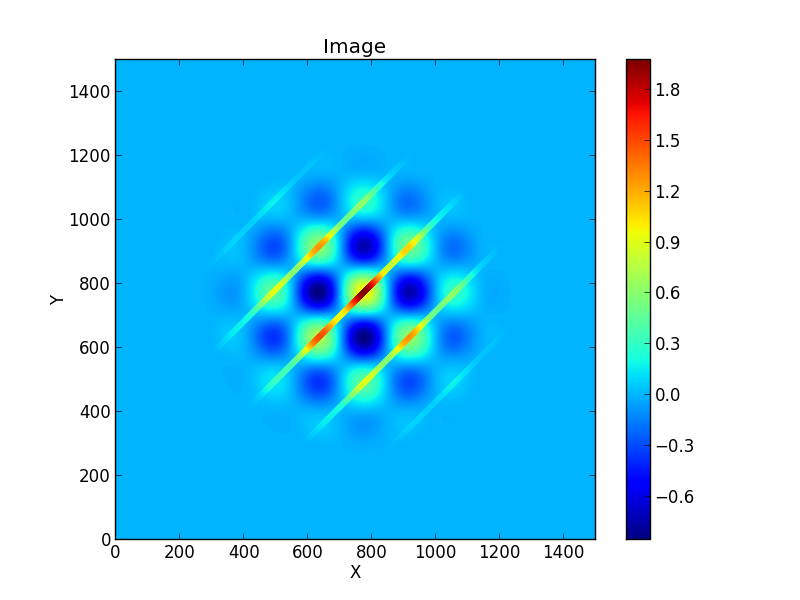
\includegraphics[width=3in]{invert_image}}
\subfloat[]{\includegraphics[width=3in]{invert_ACovF2d_nophases}} \\
\subfloat[]{\includegraphics[width=3in]{invert_ACovF1d_phases}}
\subfloat[]{\includegraphics[width=3in]{invert_ACovF1d_nophases}}
\caption{{\small
Reconstructing an image after losing information, using the ACovF (this is similar to Figure~\ref{fig:invert_psd}, but using the ACovF instead of the PSD).  
Panel a shows the original image. Panel b shows the image as reconstructed using the 2-d ACovF but a uniform random distribution of phases in the phase spectrum. Panel c shows the image as reconstructed using the 1-d ACovF but keeping the phase spectrum. Panel d shows the image as reconstructed using the 1-d ACovF and a uniform random distribution of phases (the most information loss).  In all cases, the generation of the random distribution of phases was started with the same seed value. Comparing panel b of this figure to panel b of Figure~\ref{fig:invert_psd} shows that when using the same random phase information, the reconstructed image is identical. However, comparing the bottom rows of this figure with Figure~\ref{fig:invert_psd} shows how the 1-d PSD better preserves small spatial scale information while the 1-d ACovF better preserves large spatial scale information (this is most noticeable in how panel d here is grainier than panel d in Figure~\ref{fig:invert_psd}, while panel c here better preserves the larger scale `spots' when compared to panel c in Figure~\ref{fig:invert_psd}.}}
\label{fig:invert_ACovF}
\end{figure}

In addition to evaluating the reconstructed image, we can examine the FFT, PSD or ACovF resulting from calculating these values from the reconstructed image. In particular, comparing the final 1-d PSD and 1-d ACovF or SF is interesting as these are quantities that are often used as a summary measurement in astronomy. Figure~\ref{fig:invert_compare1d} shows a comparison of the 1-d PSD and 1-d ACovF calculated from the original image compared with these quantities calculated from images reconstructed using only the 1-d PSD or 1-d ACovF with a random phase spectrum. As seen above in Figure~\ref{fig:invert_psd} and \ref{fig:invert_ACovF}, the reconstructed image in these cases does not look much like the original image. However, a 1-d PSD or 1-d ACovF calculated from these reconstructed images does still match the original 1-d PSD or 1-d ACovF fairly well (although an image reconstructed from the 1-d PSD has a better final 1-d PSD match than the image reconstructed from the 1-d ACovF, and vice versa). 

\begin{figure}[htbp]
\centering
\subfloat[]{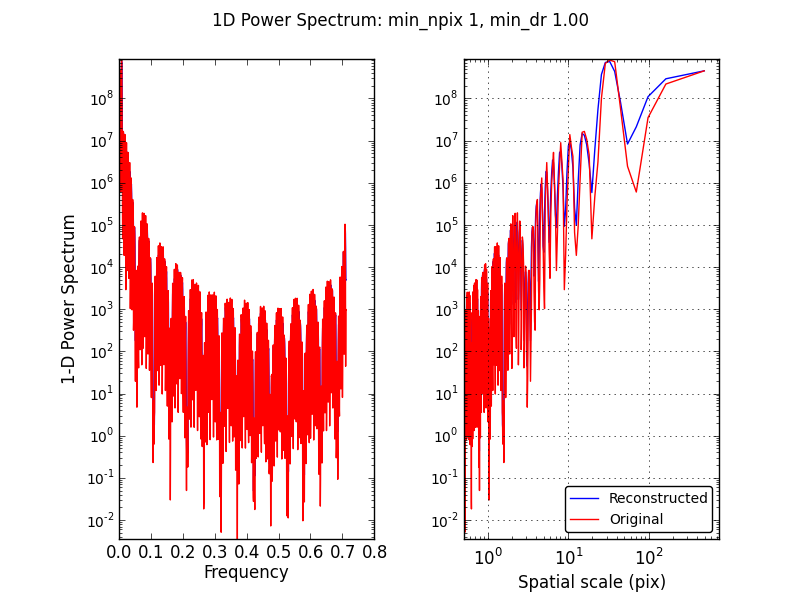
\includegraphics[width=3in]{invert_recalc_PSD_Psd1d}}
\subfloat[]{\includegraphics[width=3in]{invert_recalc_PSD_ACovF1d}}\\
\subfloat[]{\includegraphics[width=3in]{invert_recalc_ACovF_Psd1d}}
\subfloat[]{\includegraphics[width=3in]{invert_recalc_ACovF_ACovF1d}}
\caption{{\small
Calculating the 1-d PSD and 1-d ACovF from reconstructed images. These figures demonstrate the difference between the 1-d PSD and 1-d ACovF calculated from the original image and the 1-d PSD and 1-d ACovF calculated from the reconstructed images. In the top row, the image has been reconstructed from the 1-d PSD and a random phase spectrum, while in the bottom row, the image has been reconstructed from the 1-d ACovF and a random phase spectrum (in both cases, the original image was the same as in Figures~\ref{fig:invert_perfect}, \ref{fig:invert_psd}, and \ref{fig:invert_ACovF}). In each case, the 1-d PSD (or 1-d ACovF) calculated from the reconstructed image is most accurate when the 1-d PSD (or 1-d ACovF) was used to reconstruct the image. }}
\label{fig:invert_compare1d}
\end{figure}


\section{More simple images}

More simple images are available to play with using the TestImage class (testImage.py). This class gives the user the ability to add lines of varying widths, spacing and angle to the images, as in Figure~\ref{fig:example_lines_a}, or to add a Gaussian of varying sigma, or to add random noise, sine functions, or elliptical shapes. An example of the latter is shown in Figure~\ref{fig:elliptical}.  These simple test images can be used to gain some intuition on what the FFT/PSD/ACovF should look like, and the effects of inverting these values with and without the phase spectrum on the reconstructed image and/or using the 1-d PSD/ACovF. A walk-through of this process (with comments in the code) is given in example.py.

\begin{figure}[htbp]
\centering
\subfloat[]{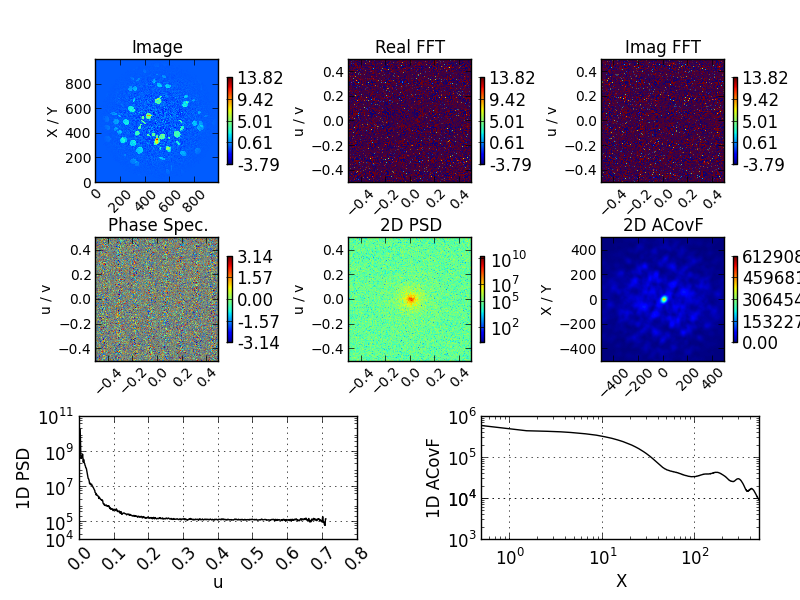
\includegraphics[width=5in]{elliptical}} \\
\subfloat[]{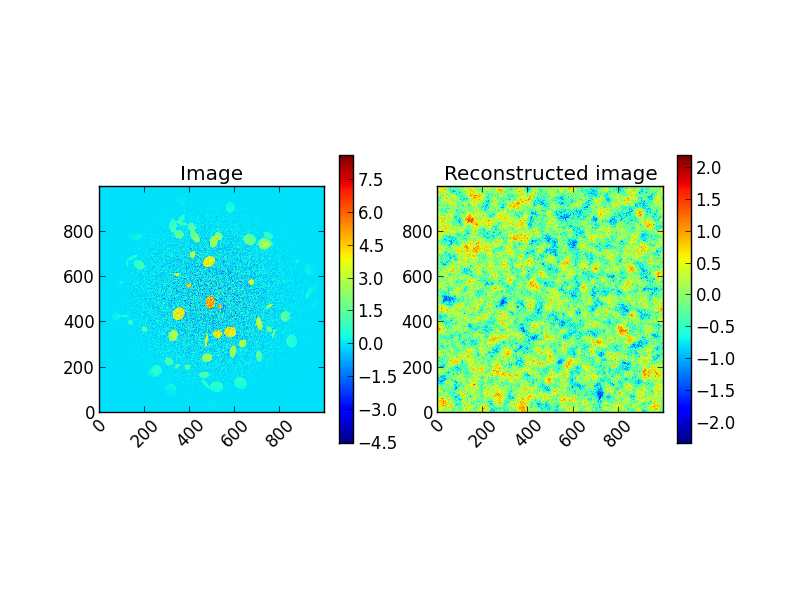
\includegraphics[width=5in]{elliptical_invert}}
\caption{{\small
An example of generating a random series of elliptical shapes, with random locations and angles, and adding gaussian white noise to the background. Panel a shows the FFT/PSD/phases/ACovF and 1-d PSD/ACovF calculated from the original image. Panel b shows the original image and the image reconstructed using only the 1-d ACovF and a random phase spectrum. }}
\label{fig:elliptical}
\end{figure}


\section{Cloud Images}

This brings us to analyzing clouds. The French calibration simulation group have provided code to generate clouds using two methods - one directly from a 1-d structure function (`old clouds') and one which is based on an 18x18 degree RASICAM image along with its extracted 2-d PSD (`new clouds').  Figure~\ref{fig:clouds_images} shows what clouds generated with each of these methods looks like. The `new' clouds end up being much more realistic looking, but we currently don't understand the physical scale related to each image. I've proceeded here under the assumption that the `windowsize' specified by the cloud generation code is in degrees, thus setting a physical scale to the overall image (in this case, the image covers 4.0 degrees), and this seems to generally agree with the overall form of the structure function (see Figure~\ref{fig:clouds_sf}).  

\begin{figure}[htpb]
\centering
\subfloat[]{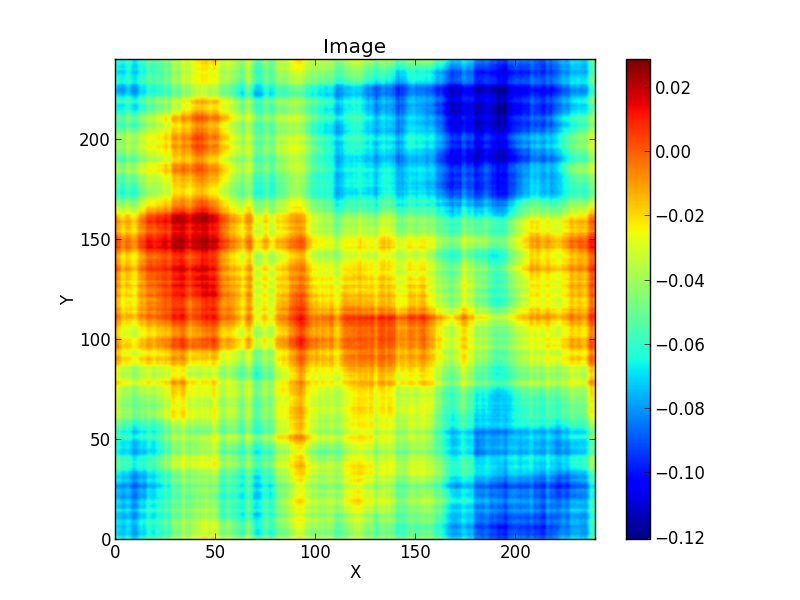
\includegraphics[width=2.5in]{clouds_oldimage}}
\subfloat[]{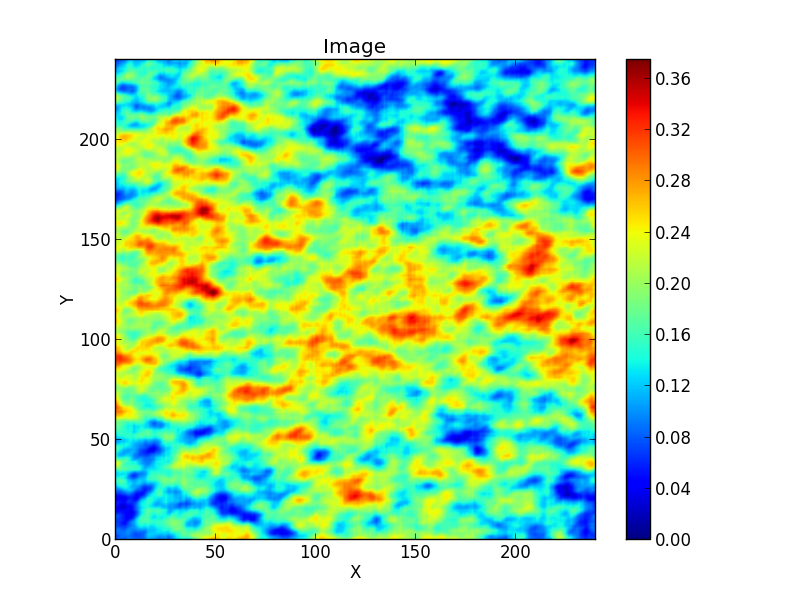
\includegraphics[width=2.5in]{clouds_newimage}}
\caption{{\small
Cloud images generated from the atmosphere\_clouds package. The images are assumed to be 4 degrees across (resulting in a pixel scale of  60"/pix). When using the images to simulate cloud extinction, the intensity variation in these images is scaled by the overall cloud extinction. Panel a shows the `old' style clouds generated from the SF only, using the code in the atmosphere\_clouds package, while panel b shows the `new' style clouds generated from a 2-d PSD generated from a RASICAM image, using the cloud from image code in the atmosphere\_clouds package.}}
\label{fig:clouds_images}
\end{figure}

Figure~\ref{fig:clouds_transforms} shows the FFT/PSD/ACovF of the old and new clouds. The old clouds have some unusual structure in the FFT and 2-d PSD which is not well understood. The new clouds have a much smoother 2-d structure in the FFT and PSD. The phase spectrum in both cases appears to be uniformly random, with no structure. A histogram of the pixel values is shown in Figure~\ref{fig:clouds_phasehist} and reinforces that the distribution appears to be uniform between $-\pi$ and $\pi$.  As noted earlier, replacing the true phase spectrum with a randomly generated one means that the overall zero point and the range of extinctions in the reconstructed image are modified. This means the `cloud extinction' values which are shown in a reconstructed image are not true extinction values, but must be scaled appropriately -- the overall gray extinction should be used to determine the mean extinction in the image, and the peak-to-peak values of the intensity should be scaled appropriately for the total gray extinction and physical scale of the image. 

\begin{figure}[htbp]
\centering
\subfloat[]{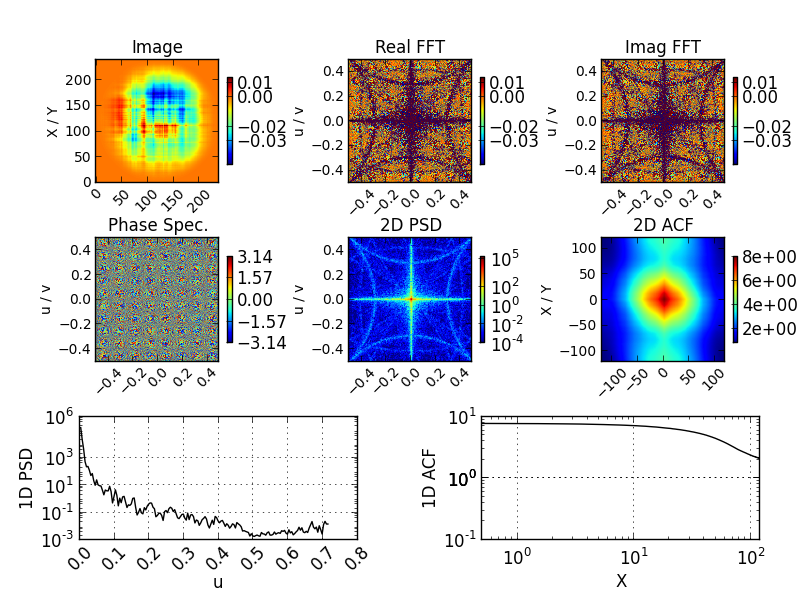
\includegraphics[width=5in]{clouds_old}} \\
\subfloat[]{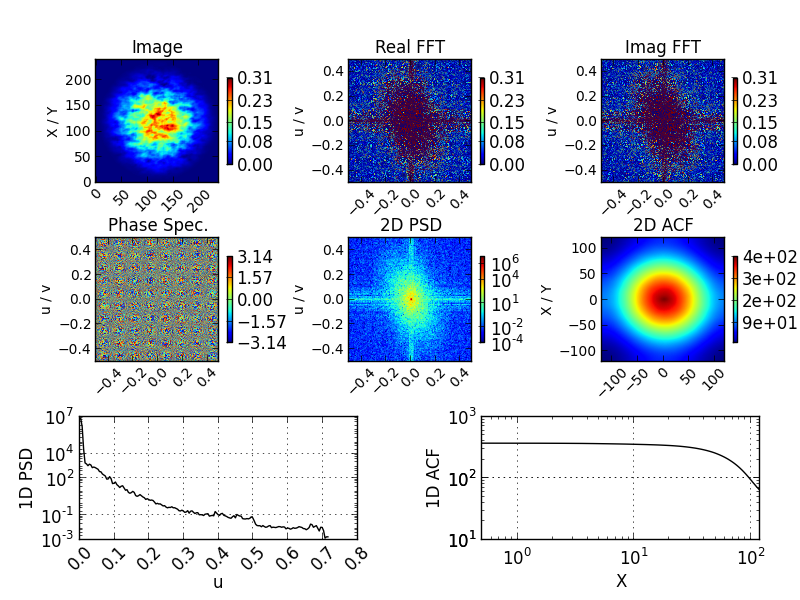
\includegraphics[width=5in]{clouds_new}}
\caption{{\small
Cloud images and their FFT/PSD/ACovF transforms, as generated from the atmosphere\_clouds package. Panel a refers to the `old' clouds, while panel b refers to the `new' clouds. The old clouds show structure in the FFT and 2-d PSD which we do not understand.}}
\label{fig:clouds_transforms}
\end{figure}

\begin{figure}[htbp]
\centering
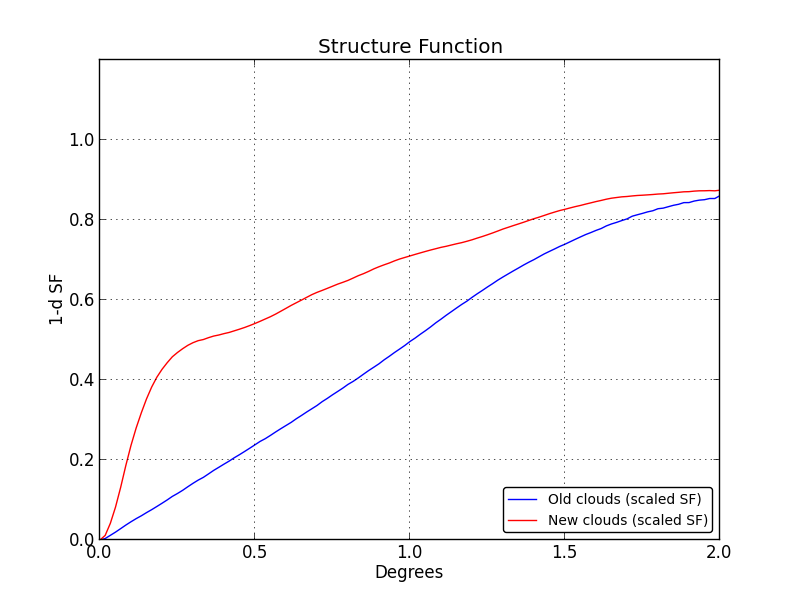
\includegraphics[width=4in]{clouds_sf}
\caption{{\small
Structure function from the `old' and `new' clouds generated from the atmosphere\_clouds package. Note that the values plotted here have been scaled to run between 0 and 1.}}
\label{fig:clouds_sf}
\end{figure}

\begin{figure}[htpb]
\centering
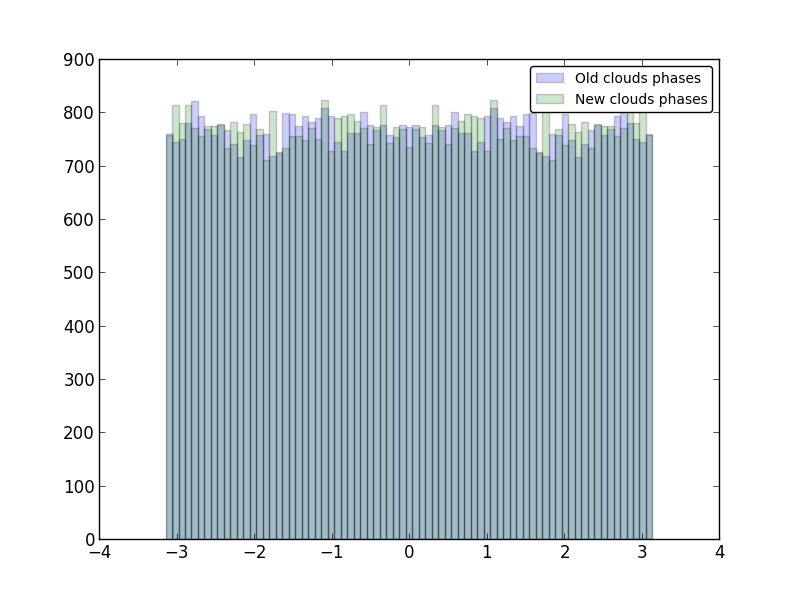
\includegraphics[width=4in]{clouds_phasehist}
\caption{{\small
Histogram of the phase spectrum, from both the old and new clouds in the atmosphere\_clouds package. }}
\label{fig:clouds_phasehist}
\end{figure}

With the tools available and described in the earlier parts of this note, I decided to attempt again to construct cloud images from the 1-d PSD used for the `old' style French clouds. I was able to determine the physical scale which seemed appropriate for the structure function (see Figure~\ref{fig:sf_degrees}), and then used this SF to reconstruct cloud extinction images, where I now know the pixel scale used to generate the image (and thus can place a physical size scale on the resulting cloud image, even if the intensities still require appropriate scaling). I generated several reconstructed images, using a different random phase distribution each time, and find distinct `cloud images' as a result. Some examples are shown in Figure~\ref{fig:clouds_newimages}.  Calculating the structure function observed in each new cloud image, I compared this with a scaled version of the SDSS structure function. The resulting structure functions are shown in Figure~\ref{fig:clouds_sf_new}, where it's clear that the final structures are close to but not identical with the original SDSS SF. The code to generate these clouds can be found in moreClouds.py. 

\begin{figure}[htpb]
\centering
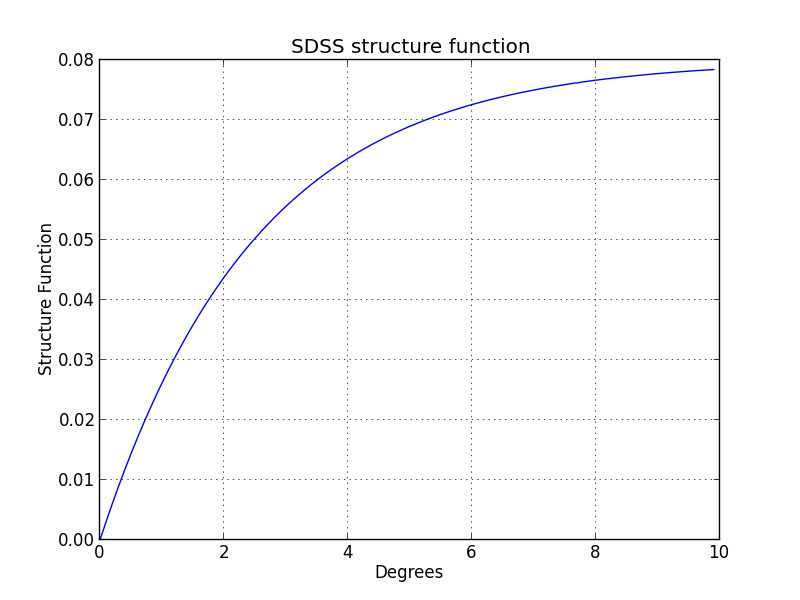
\includegraphics[width=4in]{clouds_sf_SDSS}
\caption{{\small
Input structure function based on basic structure function of `old' atmosphere\_clouds code, which seems to be from the SDSS SF.}}
\label{fig:sf_degrees}
\end{figure}

\begin{figure}[htpb]
\centering
\subfloat[]{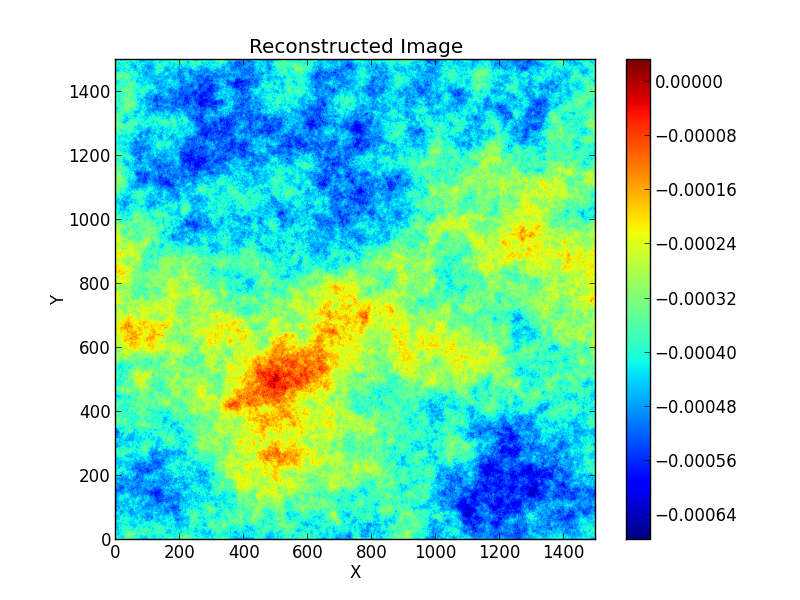
\includegraphics[width=3in]{clouds_1}}
\subfloat[]{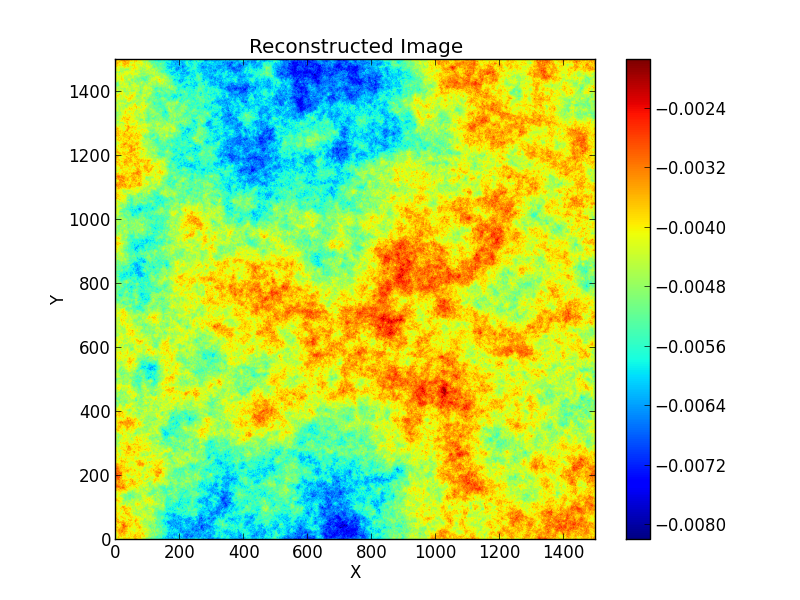
\includegraphics[width=3in]{clouds_2}}
\caption{{\small
Cloud images generated from the SDSS structure function implemented in the old style clouds above, but with an image reconstructed using the code in PImages. Panels a and b show two different realizations of clouds, where the structure function remains the same but the phase spectrum is randomly drawn each time. These images are also 4 degrees across, I understand how the physical scale of these images translates all the way from the SF, and here the resulting pixel scale is 0.00266 degrees per pixel (9.6 \arcsec / pix) (and is easily choosable by the user).}}
\label{fig:clouds_newimages}
\end{figure} 

\begin{figure}[htpb]
\centering
\subfloat[]{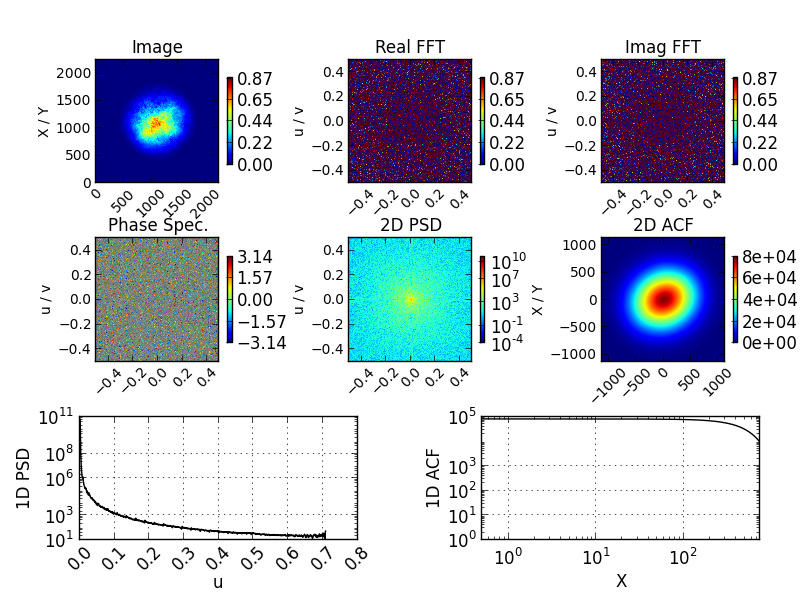
\includegraphics[width=5in]{clouds_1_dat}} \\
\subfloat[]{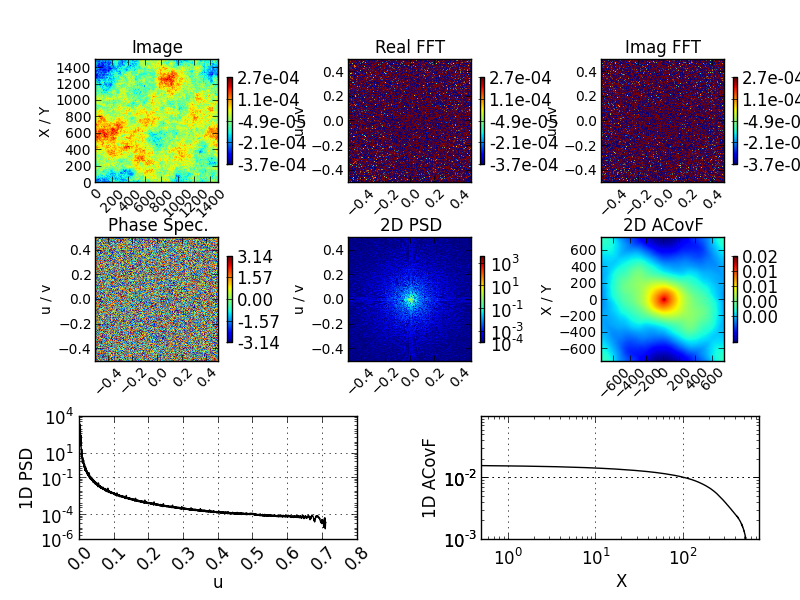
\includegraphics[width=5in]{clouds_2_dat}}
\caption{{\small
Clouds from Figure~\ref{fig:clouds_newimages} along with their FFT, PSD and ACovF.}}
\label{fig:clouds_newimages_dat}
\end{figure}

\begin{figure}[htpb]
\centering
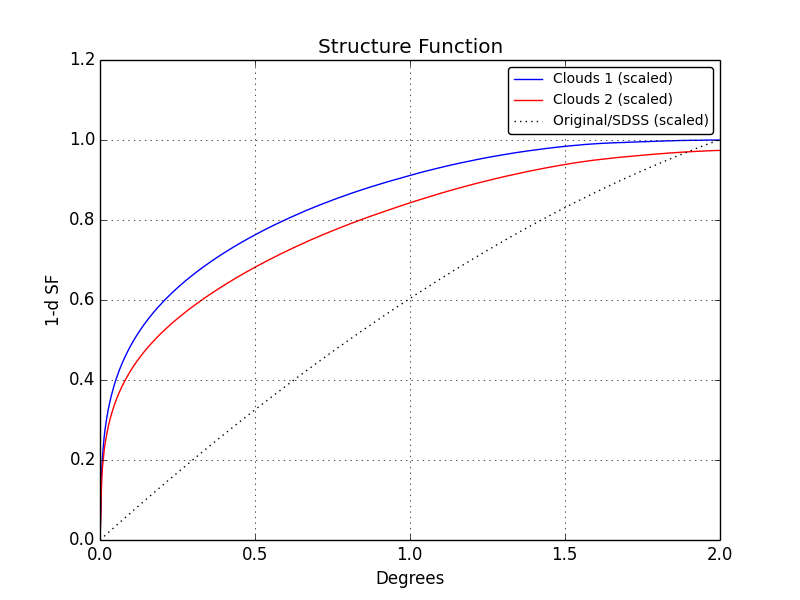
\includegraphics[width=4in]{clouds_sf_new}
\caption{{\small
Structure function from SDSS, compared with SFs calculated from reconstructed cloud images in Figure~\ref{fig:clouds_newimages}. The results are close to the original SF, but have differences (which vary from run to run, suggesting they are associated with the choice of random values for the phase spectrum).}}
\label{fig:clouds_sf_new}
\end{figure}


\section{Outstanding Questions}
\begin{enumerate}
\item{Does it make sense to place a physical scale on the 1-d PSD, and is our lack of understanding here just related to a lack of intuition on what this should show? Is a 1-d ACovF a more appropriate thing to use? (See discussion in text at \ref{q:1dpsd}).}
\item{Do these new reconstructed cloud images seem reasonable to use, given that almost anything can `kind of look like a cloud' once a random phase spectrum is added? Is it significant that the SF is not exactly recreated? Can we obtain some cloud extinction data to evaluate the phase spectrum of real clouds? Is it possible to recreate the extinction variations within the cloud extinction image appropriately, even with a random phase spectrum (since the translation from SF to extinction values seems somewhat repeatable, perhaps there is some scaling factor that just needs to be included)?}
\item{How can one go gracefully go from doing regular FFTs on a tangent plane-projection to using full spherical harmonics on the sky (for example, for evaluation of photometric zero point residuals)?}
\end{enumerate}




\end{document}

% LocalWords:  scipy FFT ps png oldclouds azimuthally newclouds FFTs
